\documentclass{standalone}
\usepackage{tikz}
\usetikzlibrary{shapes,arrows,positioning,calc,backgrounds,fit}

\begin{document}

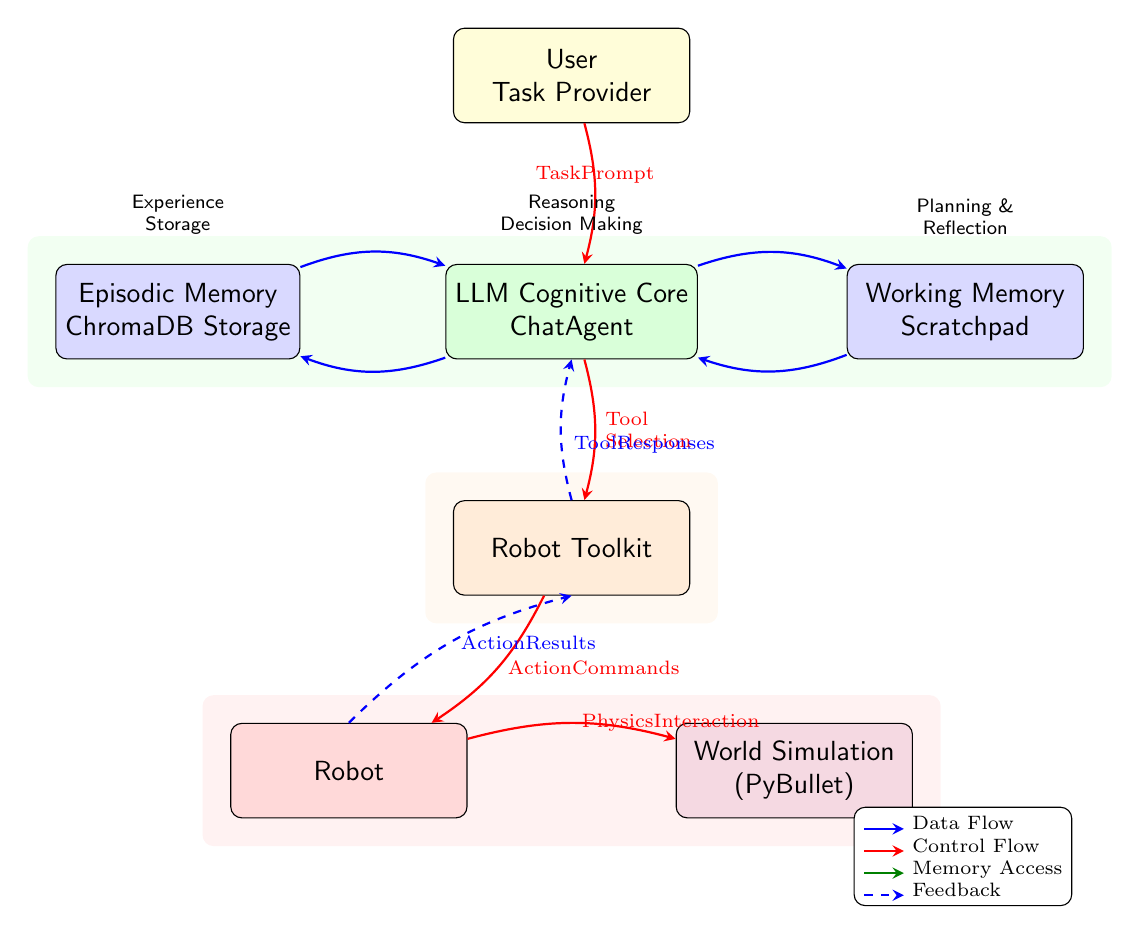
\begin{tikzpicture}[
    node distance=1.5cm and 2cm,
    box/.style={draw, rounded corners, minimum width=3cm, minimum height=1.2cm, align=center, font=\sffamily},
    layer/.style={box, fill=black!10, minimum width=4cm},
    component/.style={box, fill=white},
    memory/.style={component, fill=blue!15},
    cognitive/.style={component, fill=green!15},
    interface/.style={component, fill=orange!15},
    execution/.style={component, fill=red!15},
    environment/.style={component, fill=purple!15},
    arrow/.style={->, >=stealth, thick},
    bentarrow/.style={arrow, bend left=15},
    dataflow/.style={bentarrow, blue},
    controlflow/.style={bentarrow, red},
    memoryflow/.style={bentarrow, green!50!black},
    label/.style={font=\sffamily\bfseries, align=center}
]


% User node (external to system layers)
\node[component, fill=yellow!15] (user) at (0,9) {User\\Task Provider};

% Cognitive Layer Components
\node[cognitive, below of=user, node distance=3cm] (llm) {LLM Cognitive Core\\ChatAgent};
\node[memory, left of=llm, node distance=5cm] (memory) {Episodic Memory\\ChromaDB Storage};
\node[memory, right of=llm, node distance=5cm] (scratchpad) {Working Memory\\Scratchpad};

% Interface Layer Components
\node[interface, below of=llm, node distance=3cm] (toolkit) {Robot Toolkit};

% Execution Layer Components
\node[execution, below left of=toolkit, node distance=4cm and 4cm] (robot) {Robot};

% Environment Layer Components
\node[environment, below right of=toolkit, node distance=4cm and 4cm] (simulation) {World Simulation\\(PyBullet)};

% Connections within Cognitive Layer
\draw[dataflow] (llm) to [bend left=20] node[above, font=\scriptsize] {} (memory);
\draw[dataflow] (memory) to [bend left=20] node[below, font=\scriptsize] {} (llm);
\draw[dataflow] (llm) to [bend left=20] node[above, font=\scriptsize] {} (scratchpad);
\draw[dataflow] (scratchpad) to [bend left=20] node[below, font=\scriptsize] {} (llm);

% Connection from User to LLM (Task Input)
\draw[controlflow] (user) to [bend left=15] node[above, font=\scriptsize] {Task\\Prompt} (llm);

% Connections from Cognitive to Interface
\draw[controlflow] (llm) to [bend left=15] node[right, font=\scriptsize, align=left] {Tool\\Selection} (toolkit);
% \draw[memoryflow] (memory.south) -- ++(0,-0.5) -| node[above right, font=\scriptsize, pos=0.25] {Memory\\Access} (toolkit.north);
% \draw[memoryflow] (scratchpad.south) -- ++(0,-0.5) -| node[above left, font=\scriptsize, pos=0.25] {Reasoning\\Data} (toolkit.north);

% Connections from Interface to Execution
\draw[controlflow] (toolkit) to [bend left=15] node[right, font=\scriptsize] {Action\\Commands} (robot);

% Connections from Execution to Environment
\draw[controlflow] (robot) to [bend left=15] node[right, font=\scriptsize] {Physics\\Interaction} (simulation);

% Feedback connections (Environment -> Execution -> Interface -> Cognitive)
\draw[dataflow, dashed] (robot.north) to [bend left=15] node[right, font=\scriptsize] {Action\\Results} (toolkit.south);
\draw[dataflow, dashed] (toolkit.north) to [bend left=15] node[above right, font=\scriptsize, pos=0.25] {Tool\\Responses} (llm.south);

% Tool details (around toolkit)
% \node[below=0.3cm of toolkit, font=\scriptsize\sffamily, align=center] (tools) {
%     \begin{tabular}{c}
%         look\_around() \\
%         move\_to() \\
%         grab() \\
%         place() \\
%         search\_memory() \\
%         end\_task() \\
%         scratchpad\_ops()
%     \end{tabular}
% };

% Define layers with background rectangles that automatically resize
\begin{scope}[on background layer]
    \node[fill=green!5, rounded corners, fit=(llm) (memory) (scratchpad), inner sep=10pt, label={[label]above:Cognitive Layer}] (cognitivelayer) {};
    \node[fill=orange!5, rounded corners, fit=(toolkit), inner sep=10pt, label={[label]above:Interface Layer}] (interfacelayer) {};
    \node[fill=red!5, rounded corners, fit=(robot) (simulation), inner sep=10pt, label={[label]above:Execution Layer}] (executionlayer) {};
\end{scope}

% Annotations
\node[above=0.25cm of llm, font=\scriptsize\sffamily, align=center] {Reasoning\\Decision Making};
\node[above=0.25cm of memory, font=\scriptsize\sffamily, align=center] {Experience\\Storage};
\node[above=0.25cm of scratchpad, font=\scriptsize\sffamily, align=center] {Planning \&\\Reflection};

% Legend
\node[draw, rounded corners, fill=white, align=left, font=\scriptsize, anchor=north east] at ($(current bounding box.south east)+(-0.5,0.5)$) {
    \tikz\draw[dataflow] (0,0) -- (0.5,0); Data Flow\\
    \tikz\draw[controlflow] (0,0) -- (0.5,0); Control Flow\\
    \tikz\draw[memoryflow] (0,0) -- (0.5,0); Memory Access\\
    \tikz\draw[dashed, dataflow] (0,0) -- (0.5,0); Feedback
};

\end{tikzpicture}

\end{document}